% This is text associated with the open textbook "Open Electromagnetics"
% See immediately below for author, date
% This work is licensed under the Creative Commons Attribution-ShareAlike 4.0 International License. (CC BY-SA 4.0) 
% To view a copy of the license, visit http://creativecommons.org/licenses/by-sa/4.0/

%ORB TITLE Parallel Wire Transmission Line
%ORB AUTHOR 0        # S.W. Ellingson, Virginia Tech (ellingson@vt.edu)
%ORB DATE 20191121   # yyyymmdd
%ORB ABSTRACT  

\label{m0188_Parallel_Wire_Transmission_Line} % <-- Must match name of this file and module directory name.  Don't mess with this!
\index{transmission line!parallel wire|(}

A parallel wire transmission line consists of wires separated by a dielectric spacer.
Figure~\ref{m0188_fTwinLead} shows a common implementation, commonly known as ``twin lead.''
\index{twin lead}
The wires in twin lead line are held in place by a mechanical spacer comprised of the same low-loss dielectric material that forms the jacket of each wire.
Very little of the total energy associated with the electric and magnetic fields lies inside this material, so the jacket and spacer can usually be neglected for the purposes of analysis and electrical design. 
%
\begin{figure}[b!] % <--- "[b]" for first figure in section *only*; delete for 2nd and subsequent figures
\begin{center}
\pdftooltip{{  % note double braces
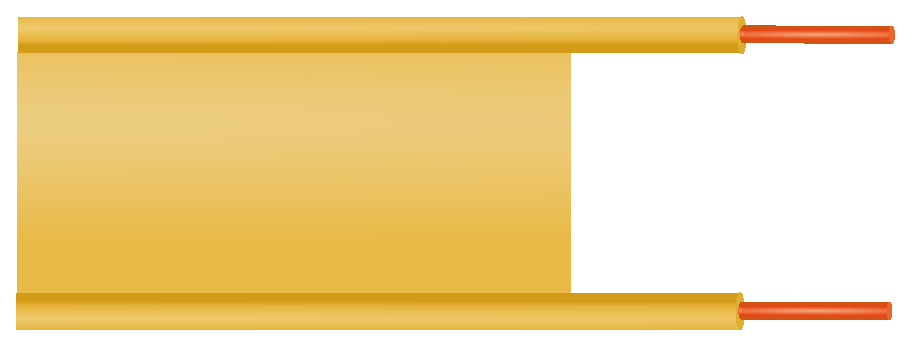
\includegraphics[width=0.7\columnwidth]{modules/m0188_fTwinLead.eps}
% https://commons.wikimedia.org/wiki/File:Twin-lead_cable_dimension.svg
}}{Two wires run parallel from left to right. The material they are encased in forms a rectangular spacer between them. The distance between the wires is uniform.}
\end{center} 
\centerline{\scriptsize 
\copyright~\hyperref[m0188_fTwinLead_Credit]{SpinningSpark, Inductiveload}  
\href{https://creativecommons.org/licenses/by-sa/3.0/}{CC BY~SA 3.0} 
(modified)
} 
\caption{
\label{m0188_fTwinLead}
Twin lead, a commonly-encountered form of parallel wire transmission line.
}
\end{figure}

Parallel wire transmission line is often employed in radio applications up to about $100$~MHz as an alternative to coaxial line.
\index{transmission line!coaxial}
Parallel wire line has the advantages of lower cost and lower loss than coaxial line in this frequency range.
However, parallel wire line lacks the self-shielding property of coaxial cable; i.e., the electromagnetic fields of coaxial line are isolated by the outer conductor, whereas those of parallel wire line are exposed and prone to interaction with nearby structures and devices.
This prevents the use of parallel wire line in many applications.

Another discriminator between parallel wire line and coaxial line is that parallel wire line is differential.\footnote{The references in ``Additional Reading'' at the end of this section may be helpful if you are not familiar with this concept.} The conductor geometry is symmetric and neither conductor is favored as a signal datum (``ground'').  Thus, parallel wire line is commonly used in applications where the signal sources and/or loads are also differential; 
\index{transmission line!differential}
common examples are the dipole antenna and differential amplifiers.\footnote{This is in contrast to ``single-ended'' 
\index{transmission line!single-ended}
line such as coaxial line, which has conductors of different cross-sections and the outer conductor is favored as the datum.} 

Figure~\ref{m0188_fParallelWireCrossSection} shows a cross-section of parallel wire line.
%
\begin{figure}% <--- "[b]" for first figure in section *only*; delete for 2nd and subsequent figures
\begin{center}
\pdftooltip{{  % note double braces
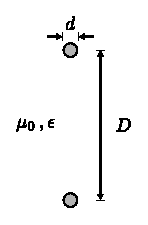
\includegraphics[width=1in]{modules/m0188_fParallelWireCrossSection.eps}
% https://commons.wikimedia.org/wiki/File:Parallel_wire_transmission_line_structure_and_design_parameters.svg
}}{Two circular cross-sections of wire, each the same size, directly one above the other. The circles' diameter is labeled small d and the distance from the center of one circle to the other is labeled capital d. Region between the wires is small mu sub zero comma small epsilon.}
\end{center} 
\centerline{\scriptsize 
\copyright~\hyperref[m0188_fParallelWireCrossSection_Credit]{C.\ Wang}  
\href{https://creativecommons.org/licenses/by-sa/4.0/}{CC BY~SA 4.0} 
} 
\caption{
\label{m0188_fParallelWireCrossSection}
Parallel wire transmission line structure and design parameters.
}
\end{figure}
%
Relevant parameters include
the wire diameter, $d$; and
the center-to-center spacing, $D$.

The associated field structure is transverse electromagnetic (TEM)
\index{transverse electromagnetic (TEM)} 
and is therefore completely described by a single cross-section along the line, as shown in Figure~\ref{m0188_fParallelLineFieldStructure}.
%
\begin{figure}
\begin{center}
\pdftooltip{{  % note double braces

\includegraphics[width=1.5in]{modules/m0188_fParallelLineFieldStructure.eps}
% https://commons.wikimedia.org/wiki/File:Electric_and_Magnetic_Field_of_Wire_Cross-Section.svg
}}{Two circular cross-sections of wire, each the same size, directly one above the other. Electric field capital e radiates from the top wire to bottom. The magnetic field intensity capital h forms a semi-circular ring around each wire.}
\end{center} 
\centerline{\scriptsize 
\copyright~\hyperref[m0188_fParallelLineFieldStructure_Credit]{S.\ Lally}  
\href{https://creativecommons.org/licenses/by-sa/4.0/}{CC BY~SA 4.0} 
} 
\caption{\label{m0188_fParallelLineFieldStructure} Structure of the electric and magnetic fields for a cross-section of parallel wire line.  In this case, the wave is propagating away from the viewer.}
\end{figure}
%
Expressions for these fields exist, but are complex and not particularly useful except as a means to calculate other parameters of interest.
One of these parameters is, of course, the characteristic impedance 
\index{characteristic impedance}
since this parameter plays an important role in the analysis and design of systems employing transmission lines.
The characteristic impedance may be determined using the ``lumped element'' transmission line model 
\index{transmission line!lumped-element model}
using the following expression:
%
\begin{equation}
Z_0 = \sqrt{\frac{R'+j\omega L'}{G'+j\omega C'}}
\end{equation}
%
where $R'$, $G'$, $C'$, and $L'$ are the resistance, conductance, capacitance, and inductance per unit length, respectively.
This analysis is considerably simplified by neglecting loss; therefore, let us assume the ``low-loss'' conditions 
$R' \ll \omega L'$ and 
$G' \ll \omega C'$.
Then we find:
%
\begin{equation}
Z_0 \approx \sqrt{\frac{L'}{C'}}~~~\mbox{(low loss)}
\label{m0188_eZ0LL}
\end{equation}
%
and the problem is reduced to determining inductance and capacitance of the transmission line.
These are
%
\begin{equation}
L' = \frac{\mu_0}{\pi}\ln\left[ \left(D/d\right) +\sqrt{\left(D/d\right)^2-1 } \right]
\end{equation}
%
\begin{equation}
C' = \frac{\pi\epsilon}{\ln\left[ \left(D/d\right) +\sqrt{\left(D/d\right)^2-1 } \right]}
\end{equation}
%
Because the wire separation $D$ is typically much greater than the wire diameter $d$, $D/d\gg 1$ and so 
$\sqrt{\left(D/d\right)^2-1} \approx D/d$.  This leads to the simplified expressions
%
\begin{equation}
L' \approx \frac{\mu_0}{\pi}\ln\left( 2D/d \right) ~~~ (D \gg d)
\end{equation}
%
\begin{equation}
C' \approx \frac{\pi\epsilon}{\ln\left( 2D/d \right)} ~~~ (D \gg d)
\end{equation}
%
Now returning to Equation~\ref{m0188_eZ0LL}:
%
\begin{equation}
Z_0 \approx \frac{1}{\pi}\sqrt{\frac{\mu_0}{\epsilon}}\ln\left( 2D/d \right)
\end{equation}
%
Noting that $\epsilon=\epsilon_r\epsilon_0$ and $\sqrt{\mu_0/\epsilon_0}\triangleq\eta_0$, we obtain
%
\begin{equation}
\boxed{
Z_0 \approx \frac{1}{\pi}\frac{\eta_0}{\sqrt{\epsilon_r}}\ln\left( 2D/d \right)
}
\label{m0188_eZ0PWL}
\end{equation}
%
%%%%%%%%%%%%%%%%%%%%%%%%%%%%%%%%%%%%%%%%%%%%%%%
%ORB HIGHLIGHT
\begin{mdframed}[backgroundcolor=yellow!20,nobreak=true] 
The characteristic impedance of parallel wire line, assuming low-loss conditions and wire spacing much greater than wire diameter, is given by Equation~\ref {m0188_eZ0PWL}.
\end{mdframed}
%%%%%%%%%%%%%%%%%%%%%%%%%%%%%%%%%%%%%%%%%%%%%%%
%
Observe that the characteristic impedance of parallel wire line increases with increasing $D/d$.  Since this ratio is large, the characteristic impedance of parallel wire line tends to be large relative to common values of other kinds of TEM transmission line, such as coaxial line and microstrip line.  An example follows.

%%%%%%%%%%%%%%%%%%%%%%%%%%%%%%%%%%%%%%%%%%%%%%%
%ORB EXAMPLE
~\\ \begin{example} 
\begin{mdframed}[backgroundcolor=brown!20,linecolor=brown!20]\raggedright
$300~\Omega$ twin-lead.
\\~\\
A commonly-encountered form of parallel wire transmission line is $300~\Omega$ twin-lead.
Although implementations vary, the wire diameter is usually about 1~mm and and the wire spacing is usually about 6~mm.
The relative permittivity of the medium $\epsilon_r\approx 1$ for the purposes of calculating transmission line parameters, since the jacket and spacer have only a small effect on the fields.
 For these values, Equation~\ref{m0188_eZ0PWL} gives $Z_0\approx 298~\Omega$, as expected.
\end{mdframed}
% note figures will need to go between "\end{mdframed}" and "\end{example}"
\end{example}
%%%%%%%%%%%%%%%%%%%%%%%%%%%%%%%%%%%%%%%%%%%%%%%

Under the assumption that the wire jacket/spacer material has a negligible effect on the electromagnetic fields, and that the line is suspended in air so that 
$\epsilon_r\approx 1$, the phase velocity $v_p$ for a parallel wire line is approximately that of any electromagnetic wave in free space; i.e., $c$.  In practical twin-lead, the effect of a plastic jacket/spacer material is to reduce the phase velocity by a few percent up to about 20\%, depending on the materials and details of construction.  So in practice $v_p\approx 0.8c$ to $0.9c$ for twin-lead line.  

%------------------------------------

{\bf Additional Reading:}
\begin{itemize}
\item ``\href{https://en.wikipedia.org/wiki/Twin-lead}{Twin-lead}'' on Wikipedia.
\item ``\href{https://en.wikipedia.org/wiki/Differential_signaling}{Differential signaling}'' on Wikipedia.
\item Sec.~8.7 (``Differential Circuits'') in S.W.~Ellingson, \emph{Radio Systems Engineering}, Cambridge Univ.\ Press, 2016. 
\end{itemize}
 
\index{transmission line!parallel wire|)}

